\chapter{CMS: evoluzione e ruolo attuale}
\label{chap:CMSEvoluzioneRuolo}

%%%%%%%%%%%%%%%%%%%%%%%%%%%%%%%%%%%%%%%%%

Il CMS (content management system) è uno software applicativo lato server utilizzato per il coordinamento e la supervisione dei contenuti presenti in un determinato sito web. L'obiettivo è semplificare la gestione di tutti i vari elementi d'interesse indipendentemente dalle reali competenze tecniche di programmazione dell'utente incaricato per la gestione.\hfill \break


\section{Cenni storici, nascita e sviluppo}
I sistemi per la gestione dei contenuti nascono negli Stati Uniti ed inizialmente furono sviluppati ad uso privato per ovviare alla problematica amministrativa del gran quantitativo di pubblicazioni prodotte all'epoca.
Nel 1995 FileNet, un'azienda con sede in Costa Mesa (California), sviluppò un software che ad oggi può essere considerato il primo e vero content management system, strutturato secondo una suite di programmi per poter gestire i documenti in tutte le sue componentistiche (ovvero dal punto di vista del workflow, della parte grafica e di quella testuale). In maniera trasversale, nello stesso anno venne fondata la Vignette Corporation, un'azienda con sede ad Austin (Texas). 
La compagnia nacque dall'intento di andare a sviluppare uno strumento che permettesse una personalizzazione ed un'accessibilità più ampia all'interno del web development e nel 1996 venne pubblicato StoryBuilder, un sistema flessibile che permetteva la gestione dei contenuti su larga scala.
Durante il deployment, l'azienda texana strinse una collaborazione con CNET (abbreviazione di Computer Network), un sito web americano specializzato nella pubblicazione di articoli a tema tecnico-informatico, che nel contempo si mobilitò per sviluppare il proprio sistema di gestione dei contenuti, in seguito denominato PRISM, che introdusse l'utilizzo del database per la gestione interna dei dati. 
La svolta, in termini concettuali, avvenne nel 1998 quando la Pencom Web Works, una compagnia operante nel campo della consulenza aziendale, introdusse l'utilizzo del server di trasformazione dati (DTS) Metaphoria, che permise agli sviluppatori java la scrittura di applicazioni con corrispettivo collegamento dei contenuti (e distribuzione degli stessi) all'interno di canali differenti.
Il progetto non si affermò nel mercato di riferimento, ma gettò le basi per il proseguo e l'evoluzione dei content management system.
Il ventunesimo secolo segnò la definitiva consacrazione dei CMS, il tutto grazie all'avvento dei framework e la continua evoluzione dei linguaggi di programmazione che permisero alle strutture di evolversi e diventare più accessibili. Nel 2003, presero piede diversi sistemi sviluppati in ottica open source (e.g. WordPress, SquareSpace) con diretta integrazione dei template.
Il progresso che i CMS stavano affrontando viaggiava a pari passo con l'evoluzione di tutti gli apparati che permettevano l'accesso al World Wide Web e ai siti in esso contenuti. Nel 2010 venne introdotta la tecnica del design responsivo per l'adattamento automatico degli elementi grafici secondo il dispositivo al di sopra del quale venivano visualizzati i contenuti. Quest'ultima pratica permise di semplificare ulteriormente l'esperienza dell'utente nell'interagire con il sito, svincolando lo stesso dal dover riadattare eventuali entità per una migliore comprensione.
%%%%%%%%%%%%%%%%%%%%%%%%%%%%%%%%%%%%%%%%%

\section{Impatto odierno}
Nel corso degli anni, le richieste della clientela in termini di complessità e specificità per lo sviluppo di un sito web sono aumentate in maniera considerevole.
Oggi giorno, i content management system mettono a disposizione funzionalità utopistiche se messe a confronto con quelle dei suoi predecessori. La gestione dei contenuti risulta altamente semplificata, la piattaforma mette a disposizione solide basi per poter operare in totale tranquillità, i siti vengono sviluppati secondo i concetti del responsive web design (RWD), della personalizzazione per quanto ne riguarda le attività e l'estetica, dell'utilizzo multiutente con corrispettiva gestione dei permessi e del posizionamento, in riferimento all'ottimizzazione dei contenuti e delle performance, nel contesto dei motori di ricerca. \hfill \break
In termini statistici, secondo uno analisi redatta dal sito specializzato nello studio dell'utilizzo di diversi applicativi w3techs.com, circa il 52\% dei siti  utilizza un sistema per la gestione dei contenuti, dato che va a sottolineare l'ulteriore l'impatto che i CMS hanno avuto e hanno all'interno dell'online web. 
\clearpage
\subsection{CMS Open source}
Il termine open source, indica un tipo di software che, per mezzo di una licenza approvata dai proprietari, è favorevole alla modifica, allo studio, l'utilizzo e la redistribuzione del codice sorgente che per condizione implicita, è di dominio pubblico. \hfill \break
Quest'ultima caratteristica, è in parte alla base dei vantaggi offerti da questo tipo di soluzione: l'ampio numero di sviluppatori permette di tenere il sistema in costante aggiornamento mediante l'integrazione di plug-in per lo svolgimento di specifici compiti in merito all'elaborazione e della gestione dei dati e sia nello sviluppo della parte grafica, secondo l'utilizzo di appositi template per un avvio rapido e preconfigurato del sito. Il libero accesso al codice sorgente rappresenta anche la prima vulnerabilità per quanto ne concerne questa tipologia di CMS: dal punto di vista della sicurezza il sistema è vulnerabile ad eventuali attacchi di utenti malintenzionati (strutturati sulla base delle conoscenze a disposizione) e l'intervento per ovviare ad eventuali bug oppure a delle problematiche interne al software non è sempre immediato ed è a discrezione della disponibilità degli sviluppatori.
Oggi giorno, il mercato mette a disposizione diverse soluzioni: WordPress, con una copertura in termini assoluti del 30\% circa dei siti presenti online, detiene attualmente il primato in merito allo sviluppo dei siti web. Seguono diversi competitors meno famosi ma altrettanto validi come Joomla, Drupal e Squarespace, utilizzati in percentuale minore ma con una resa, in termini prestazionali, non indifferente.
\clearpage
\subsection{CMS Proprietario}
Con l'appellativo "proprietario", si fa riferimento al fatto che il CMS sia di detenzione privata nel rispetto dell'azienda o del singolo programmatore che ne ha svolto lo sviluppo in toto. Tra le principali caratteristiche, emerge il fatto che il codice sorgente sia al sicuro e non di disponibilità pubblica (a differenze della categoria antecedente). In riferimento ai vantaggi, questo tipo di soluzione mette a disposizione la possibilità di poter realizzare un sito secondo esigenze specifiche del cliente ed ovviare ad eventuali problematiche in maniera rapida ed efficiente attraverso un consulto con il proprietario del sistema. Non mancano gli svantaggi, ovvero il vincolo che si va ad instaurare con la web agency d'interesse in termini di costo/flessibilità e le limitazioni imposte dal CMS per quanto ne riguarda la scelta dei temi in ambito grafico e delle funzionalità, nel contesto dell'operatività, messe a disposizione.\hfill \break

\begin{figure}[ht!]
    \centering
    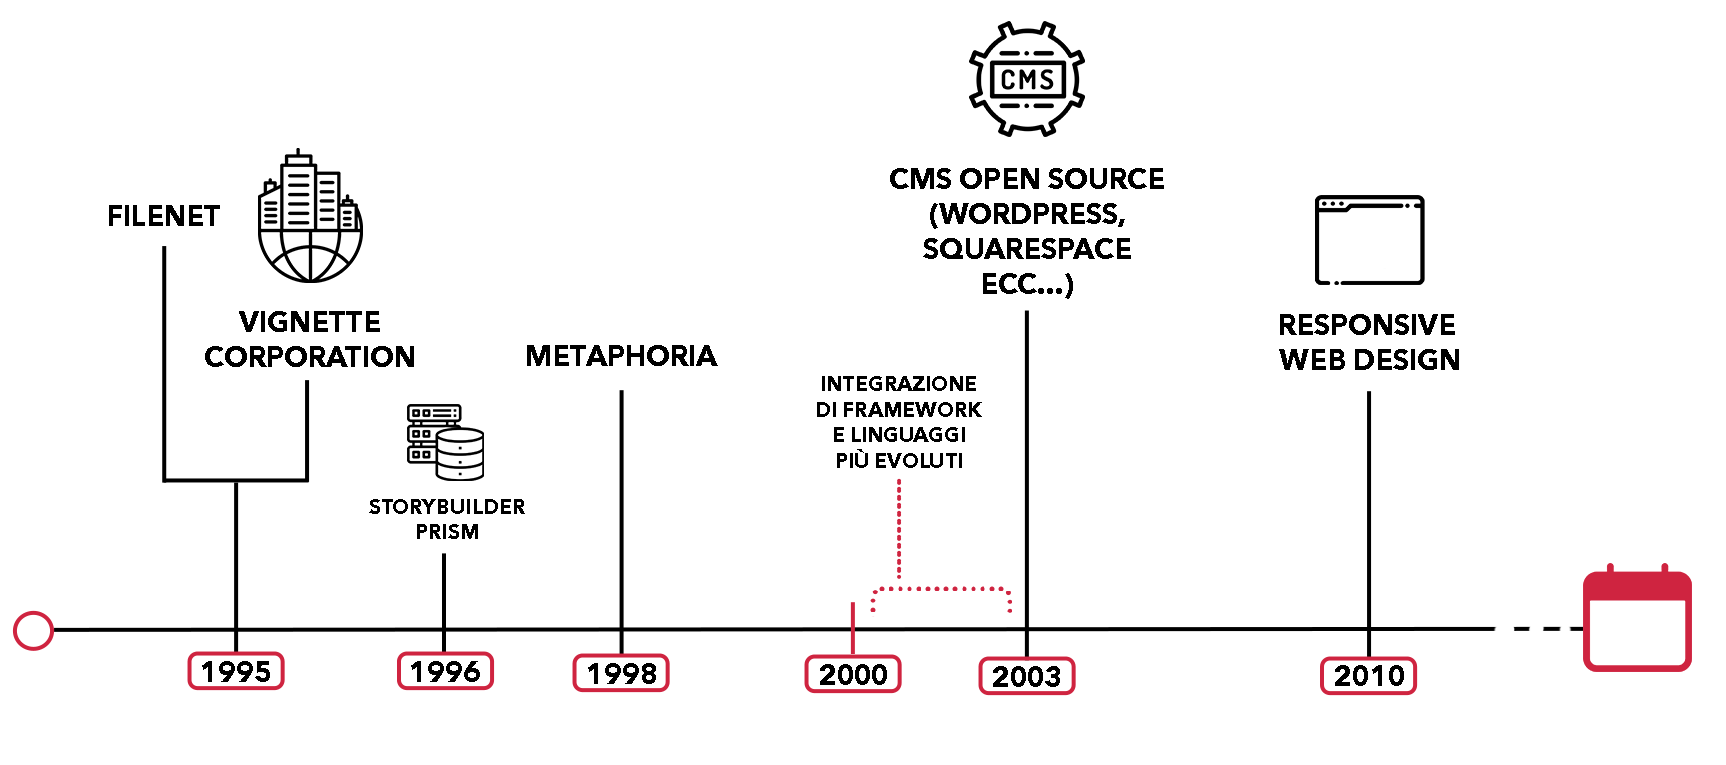
\includegraphics[width=140mm]{images/Storyline.png}
    \caption{Flusso temporale degli eventi\label{overflow}}
\end{figure}

